\documentclass[11pt,onecolumn]{article}
\usepackage[T1]{fontenc}
\usepackage{times}
\usepackage[hscale=0.8,vscale=0.9]{geometry}
\usepackage[parfill]{parskip}
\usepackage{amsmath}
\usepackage{amsfonts}
\usepackage{graphicx}
\usepackage{subfigure}
\usepackage{wrapfig}
\usepackage{amssymb}
\usepackage{enumitem}

\newcommand{\eat}[1]{}
\setlength{\textheight}{9.05in}
\setlength{\textwidth}{6.5in}
\setlength{\topmargin}{-0.5in}		% -0.5
\setlength{\oddsidemargin}{0in}
\setlength{\evensidemargin}{0in}

%\setlength{\columnsep}{0.2in}   % mike added this

% \setcounter{topnumber}{1}       % another mike: one fig/plot per column
% \setcounter{bottomnumber}{0}    % another mike: and only at the top

% \flushbottom  % Probably not good except for two-side option (facing pages)
% \raggedbottom	% In two-column mode doesn't look so good.

% \parskip .5ex
% \itemsep=-10pt

\makeatletter
%as Latex considers descenders in its calculation of interline spacing,
%to get 12 point spacing for normalsize text, must set it to 10 points
%\def\@normalsize{\@setsize\normalsize{12pt}\xpt\@xpt
%\abovedisplayskip 10pt plus2pt minus5pt\belowdisplayskip \abovedisplayskip
%\abovedisplayshortskip \z@ plus3pt\belowdisplayshortskip 6pt plus3pt
%minus3pt\let\@listi\@listI} 

%need an 11 pt font size for subsection and abstract headings
\def\subsize{\@setsize\subsize{12pt}\xipt\@xipt}

%make section titles bold and 12 point, <2 blank lines before, <1 after
\def\section{\@startsection {section}{1}{\z@}{18pt plus 2pt minus 2pt}
{6pt plus 2pt minus 2pt}{\large\bf}}

%make subsection titles bold and 11 point, 1 blank line before, 1 after
\def\subsection{\@startsection {subsection}{2}{\z@}{12pt plus 2pt minus 2pt}
{3pt plus 2pt minus 2pt}{\subsize\bf}}

\def\subsubsection{\@startsection {subsubsection}{3}{\z@}{11pt plus 2pt minus 2pt}
{3pt plus 2pt minus 2pt}{\normalsize\bf}}

% \def\subsubsection{\@startsection {subsubsection}{3}{\z@}  
%  {11pt plus 2pt minus 2pt}
%%  {3.25ex plus 1ex minus .2ex}
%  {-1em}
%  {\reset@font\normalsize\bf}
%}

\makeatother

\begin{document}
\include{weld-defns}
\title{Open-domain Knowledge Extraction}
\author{Niranjan Balasubramanian}
\maketitle
\newpage
\noindent
\thispagestyle{empty}
%!TEX root = main.tex
\begin{center}\textbf{Project Summary}\\
Niranjan Balasubramanian (PI)
\end{center}
%\author{Niranjan Balasubramanian}
\eat{
Each proposal must contain a summary of the proposed project not more than one page in length. The Project Summary consists of an overview, a statement on the intellectual merit of the proposed activity, and a statement on the broader impacts of the proposed activity.
The overview includes a description of the activity that would result if the proposal were funded and a statement of objectives and methods to be employed. The statement on intellectual merit should describe the potential of the proposed activity to advance knowledge. The statement on broader impacts should describe the potential of the proposed activity to benefit society and contribute to the achievement of specific, desired societal outcomes.
The Project Summary should be written in the third person, informative to other persons working in the same or related fields, and, insofar as possible, understandable to a scientifically or technically literate lay reader. It should not be an abstract of the proposal.
}
\eat{Textual information sources are typically authored for human consumption and therefore assume a level of background knowledge and 
inference capacity that is beyond the reach of current information extraction systems. A basketball article might assume which Michael Jordan one is talking about, an article on a genome will assume what gene a RF32 refers and so on. Even news articles written eaves many other dots that a human reader would implicitly and effortlessly connect. This knowledge is extremely difficult to attain. This project aims to extract this background knowledge about events and entities of the world to help extraction and summarization systems produce riche yet concise representations of information in texts. }

\eat{Existing information extraction systems do not have access to this kind of knowledge. Open IE systems extract every (binary) relation mentioned in text with no notion of salience or structure. Template-based IE systems aim to extract information into a richer structure but depend on manually specified templates, which result their applicability to a small set of domains. Prior work on automatic generation lead to a scalable method for producing schemas. However, the quality of the resulting schemas were lacking. The schemas were largely incoherent schemas that often mixed distinct events and roles. The light-weight subject-verb or verb-object representation improved robustness of estimates but often missed essential context. Our own preliminary work in this area showed that it is possible to use a richer representation and address the resulting sparsity issues with some simple generalization techniques. }

	
\eat{The project will proceed in three phases. In the first phase of the project, we focus on the designing the representation and extracting information from large corpora using existing IE systems. We will design a rich representation for the targeted knowledge by leveraging existing ontologies for entities and relations (e.g., YAGO, NELL, Freeebase) where possible and using text derived representations in other places. Then, we will investigate techniques for aggregating and generalizing information in the specific instances. In particular, we will develop automatic methods for choosing the right level for mapping into a type hierarchy for the arguments and the relations. In the second phase, we will focus on graph-based approaches for generating open-domain schemas using the generalized extractions. In our preliminary work, we identified the graph properties that indicate specific characteristics for good schemas and developed a suitable method that exploited the graph properties to produce high-quality schemas. In the third phase, we will focus on applying the generated schemas to two end tasks: event extraction, and summarization. For event extraction we will build extractors. Schemas can be thought of as high-precision models of events, which can then be expanded to include higher-recall extractors via bootstrapping. For summarization, we will use schemas to help select sentences for the standard MUC single document summarization task. We will iterate and refine the schema representation and generation based on their performance in these end tasks. }

Information extraction systems are critical for mining useful information from the massive amounts of texts available on the web. Textual sources written for human consumption raise two types of challenges for extraction systems: (i) They include many non-relevant information (e.g., ``Bill gates, {\em the father of two}, founded Microsoft ..."), and (ii) They exclude some useful information, expecting the reader to have a level of background knowledge or inference capacity. For example, a basketball article might assume which {\em Michael Jordan} one is talking about, an article on a genome will assume what gene a {\em RF32} refers to and so on. Existing information extraction systems do not have access to this kind of open-domain knowledge. Open IE systems extract every (binary) relation mentioned in text with no notion of salience or structure. Template-based IE systems aim to extract information into a richer structure but depend on manually specified templates, which result their applicability to a small set of domains.

The main goal of this project is to investigate scalable methods for producing high-quality open-domain knowledge about events and their effective application to event extraction and summarization. Building on our preliminary work on event schemas, we will target effective representations with adequate generalization, and scalable graph-based methods for identifying schema elements. We will leverage existing Open IE extractors, as well as knowledge-bases such as Freebase, YAGO, and NELL to produce a rich and effective representation. These schemas will specify the typical participants in an event, their roles, and the dependencies between various sub-events. To keep our investigation grounded, we will iterate on the design and development focusing on two end tasks {\em event extraction} and {\em summarization}. %First, we will transform the schemas into effective extractors by developing methods for expanding the schemas to include extraction patterns.  Second, we will improve state-of-the-art summarization systems by injecting a model of salience for entities, sub-events and their dependence derived from schemas. , 

{\bf Intellectual Merit} Through the course of this project, we will have made significant contributions in generating knowledge about open-domain events. Our first contribution will be in representing events using a combination of information from multiple sources and effective mechanisms for generalizing from specific event mentions. A second fundamental contribution would be the exploration of probabilistic graphical formalisms for identifying clusters of relations that correspond to an event. This involves contributions in methodology for constructing large relation graphs, encoding relevant phenomena via graphical properties, and algorithmic adaptations to score the desired clusterings. The third major contribution of this work would be novel techniques for expanding relation extractors from a high-precision seed set. \eat{Unlike prior approaches for event template construction where schema specific documents were gathered first, we will focus on an approach that will construct schemas first and then identify schema specific documents later to expand.}The fourth major contribution here would be methods for estimating models of salience and dependence between schema elements and empirical evaluations of the utility of the information in event schemas for {\em event extraction} and {\em summarization}.

%understanding of the representation needs for event schemas in relation to event extraction and summarization and demonstration of the value of schema like knowledge for these tasks. The method and techniques can scale to and spur research on similar problems in other domains (e.g., extracting processes from textbooks, identifying schemas in research studies). 


{\bf Broader Impact} 

Extracting and summarizing information is a central to knowledge acquisition and organization, which has direct societal benefits and impacts many different communities including business intelligence, scientific research community, as well as the Artificial Intelligence community. All these diverse communities can benefit from scalable information extraction and summarization systems. Event schemas are an important step towards automatically building script-like knowledge from text, which can benefit knowledge-intensive applications such as reasoning and Question Answering, which further the cause of Artificial Intelligence. 

{\bf Keywords} Knowledge extraction, Information extraction, Event extraction, Summarization

%\end{document}
     % A. Project Summary - 1 page
\newpage
\tableofcontents    % B. Form 1359
\thispagestyle{empty}
\setcounter{section}{0}
\setcounter{page}{0}

\newpage
%
\setcounter{page}{1}
% !TEX root =  main.tex
\section{Introduction}
\subsection{Motivation}

Building systems that can understand and reason with information present in texts is a central pursuit in the AI vision. Extracting from texts is a challenging task in itself and requires access to open-domain knowledge. It is no surprise that these articles written for human consumption assume background knowledge and an inference capability that reads between lines. For example, consider extracting information from the following news snippet:

\begin{verbatim}
        Somalia's al-Shabab militant group has confirmed the death 
        of its leader in a U.S. airstrike and named his successor. 
        The al-Qaida linked militants announced the selection of 
        Abu Ubeid Ahmed Omar to replace Abdi Godane. 
\end{verbatim}

Extraction systems need to be told what information to extract -- e.g, the one who gets replaced, the successor, the position being filled, the employing organization etc. Reading these two sentences, we can easily determine the important information: {\em Abdi Godane} was the leader of {\em al-Shabab}, which is a {\em terrorist group} and {\em Abu Ubeid Ahmed Omar} is the successor of {\em Abdi Godane}, and {\em Abdi Godane} was killed by a {\em U.S.} airstrike.  Further, none of this information is explicitly mentioned in the sentences. Further This kind of declarative knowledge in terms of the participants and their roles (e.g., the one who gets replaced, the successor, the position, the organization etc.) also provides constraints that can help resolve ambiguities and also extract implicit connections. Further such knowledge can also provide effective guidance for producing effective summaries. 

Existing state-of-the-art information systems do not have access to this kind of open-domain knowledge.
For example, Open information extraction (Open IE) systems extract {\em every} possible binary relation explicitly stated in text because they do not have any notion of salience. Moreover, most events and scenarios involve multiple participants with specific roles that are not effectively represented by binary relations. 

Template-driven extraction aims to address these issues by pre-specifying an extraction template or a schema for each event type (e.g., arrest, arson, bombing). 
The schema describes an event type in terms of the actors and the roles they play within the event. %Figure~\ref{fig:arrest} shows an example.  
\eat{\begin{wrapfigure}{lhb}{0.5\textwidth}
	\vspace{-2ex}
	\begin{center}
	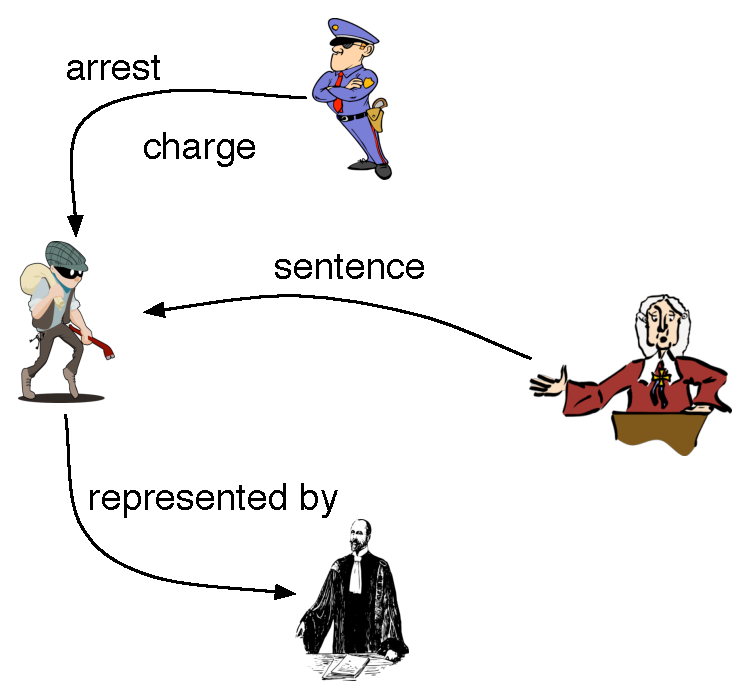
\includegraphics[width=1.5in,height=1in]{figures/arrest-schema} 	
	\caption{\label{fig:arrest} {Arrest schema: A model for an arrest scenario with the key actors and their roles.}}
	\vspace{-3ex}
	\end{center}
\end{wrapfigure}}
For example, the key participants in a arrest event are an arresting agent who arrests and charges a suspect, a lawyer and a judge who rules on the case. However, template-based information extraction has been largely limited to a handful of domains. Prior automatic methods for generating event schemas~\cite{chambers-acl09} suffer from coherence issues -- mixing distinct events (e.g, fire spreading vs. disease spreading). 

The lack of event schemas covering a broad range of domains and the difficulty of acquiring them manually is a fundamental challenge in scaling event extraction. 

%Chambers and Jurafsky (2009) developed an automatic method for generating event schemas that scaled to arbitrary domains but used a simple representation that resulted in schemas that were mostly incoherent because they mixed distinct events (e.g., fire spreading vs. disease spreading). 

\subsection{Proposal}
In this work, I propose to tackle the main challenges in schema-based event extraction by developing methods for automatically generating event schemas and produce a large scale curated collection of schemas to promote further research. In particular, I will target generation of schemas that specify the participants (actors) and their roles via generalized relations with semantically typed arguments. Figure~\ref{fig:drug-schema} shows an example that represents information about a scenario where a player gets suspended for taking a drug. The key participants include the player, the drug used, the test they failed and the punishment. The relations indicate the roles the participants play.  

First, I will develop representations and algorithms for automatically generating open-domain event schemas. I will investigate corpus-based techniques that exploit relation co-occurrence to identify generalized relations that belong in a schema. This involves handling significant research challenges in a) generating effective representations while also addressing the resulting sparsity issues, and b) building effective graph-based algorithms that can identify clusters of co-mentioned relations. Second, I will also develop techniques to build extractors using these event schemas. The main scope of this activity is to keep the schema generation effort grounded in this end task and to demonstrate the feasibility of open-domain event extraction, Third, I propose to create a large scale curated collection of automatically generated open-domain event schemas (~10K) and an event extraction dataset.
\begin{figure}[thb]
	\begin{center}
	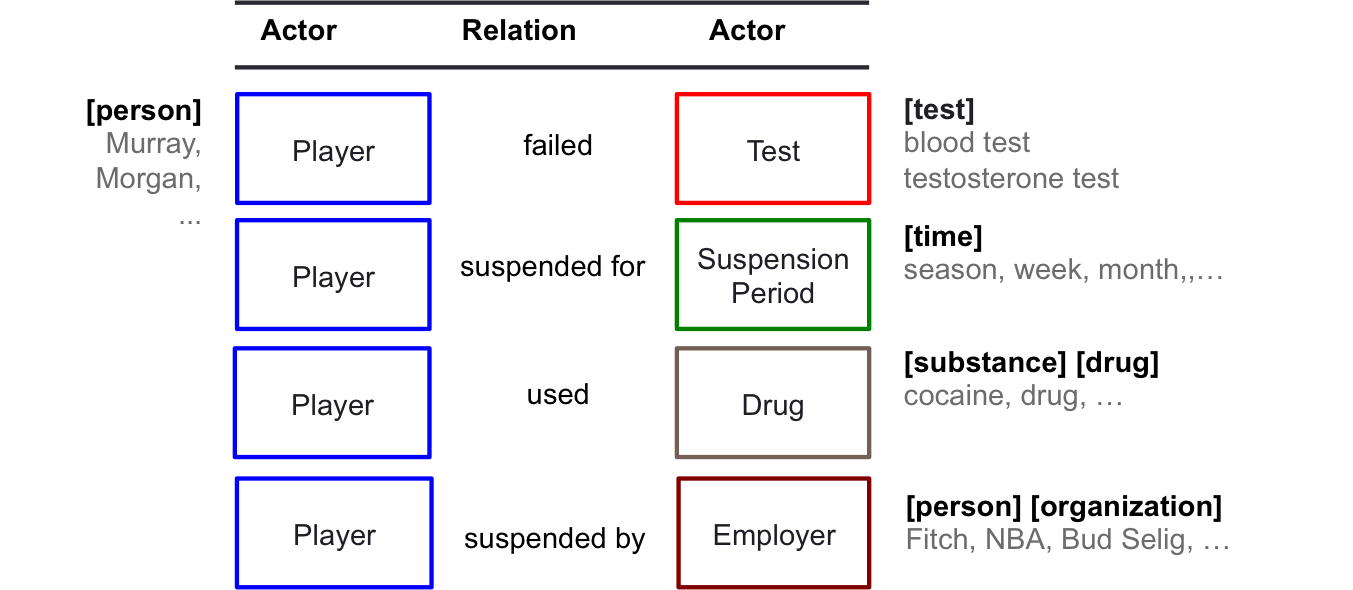
\includegraphics[width=5.7in,height=2.5in]{figures/drug-schema} 	
	\caption{\label{fig:drug-schema} {Drug Suspension Schema, which specifies the participants (actors) involved and their roles. The square boxes represent the participants. The semantic types of the participants are shown by their side along with some example instances for each participant.}}
	\vspace{-2ex}
	\end{center}
\end{figure}
%The key research challenges include designing an effective representation -- There is an inherent trade-off in choosing a the smallest units to use for representing information about events. Include more contexts reduces ambiguity but also increases sparsity. Representations that are closer to text provide less generalization power due to syntactic and lexical variability.
%\item Schema Generation -- Determining the starting points for building good schemas, and 
%\item 
%\end{enumerate}


\subsection{Contributions}
The proposal builds upon the initial results and key findings in our prior work for automatically generating coherent event schemas~\cite{balasubramanian-akbc12,balasubramanian2013generating}. Exploiting recent advances in relation extraction technology, as well as large scale resources (e.g., NELL, Freebase), I will target automatic generation of high quality event schemas and release large scale datasets to further event extraction research. 

Successful completion of the proposed activities will make the following technical contributions:
\begin{itemize}[noitemsep,nolistsep]
\item An effective representation for events that reduces ambiguity and techniques to address sparsity.
\item Graph-based approaches that use graphical properties to address topic-drift in order to produce high-quality schemas.
\item Effective bootstrapping techniques for building extractors for schema elements.
\item  A large scale collection of manually curated open-domain schemas and large scale evaluation data set for event extraction that covers a wide range of domains.
\end{itemize}
\newpage


\eat{
In this work, we target extraction of rich event schemas that describe events using a range of information as shown in the table below.
\begin{table}[htdp]
\caption{default}
\begin{center}
\begin{tabular}{|p{4cm}|p{12cm}|}
\hline
Entities & Extractors\\
& Researcher, Organization, Subject, Problem, Conclusion, Publication, Date, Location \\
\hline
Sub-events &  \\
& R: Researcher study Problem (X)\\
& R find found/discovered/uncovered/stumbled/ Conclusion (Y) \\
& R published Results/Conclusions in [Journal/Book/Conference] \\
& R supports/refutes \\
& \\
\hline
Background-relations & \\
& R: Researcher, employed by, O:[Organization] \\
& study: Research, funded by, O:[Organization] \\
\hline
Entity Extractors & \\
& X:[Person] studies Y: [Problem] $\rightarrow$ X: [Researcher] \\
& X is studied by Y: [Person] $\rightarrow$ X: [Subject]\\
& X: [Researcher] concludes Y $\rightarrow$ Y: [Conclusion]\\
\hline
Relation Extractors & \\
	& study -- studied, investigated, explored, asked\\
	& find -- discovered, uncovered, stumbled \\			
\hline
Dependencies (Rel-grams) & \\
& R found Y, Conclusion(Y) $\rightarrow$ R publishes Y \\
& R found Y, Conclusion(Y) $\rightarrow$ R studied X \\	
\hline
Related Scripts & \\
& investigate, publish \\
\hline
\end{tabular}
\end{center}
\label{default}
\end{table}%

}


%To effectively address these issues, extraction systems need background knowledge that provide models or expectations for the information they need to extract. For example models of salient aspects of certain types of entities (e.g., actors {\em act in} movies, actors {\em win} awards) can help extract and organize information about people. Similarly, rich descriptions of events or scenarios, processes and their interactions can help in extracting and understanding information about events from texts. Scalable methods for acquiring such background knowledge is essential for building broad coverage extractors.

%These open-domain event schemas are but a starting point for aggregating and organizing background knowledge about events that can be leveraged during extraction. The main goal of this project is to build open-domain script like knowledge about events. 

%Script-like knowledge serve as general purpose description of events or scenarios. In addition to the key actors, their actions, we will build scripts that include causal, temporal and dependency relationships between the different actions. During extraction this richer representation will enable us to infer more than what is explicitly mentioned in the text. 

%Schemas provide a high precision model of scenarios which can be expanded to associated extractors -- i.e., patterns that can be used to extract from new texts. Resolving entity and event co-references. Third, scripts must include causal and temporal ordering of the actions in a scenario. 

%\subsection{Research Challenges}
%\subsection{Contributions}

% !TEX root =  main.tex
\section{Background}

Template-driven 

\subsection{MUC Templates}



\subsection{Automatic Methods}

\textbf{C \& J, 2009}

\textbf{C \& J, 2011}

\textbf{C \& J, 2013}

\textbf{Poon et al, 2013}


\subsection{Preliminary Work}

\textbf{Rel-grams}

\textbf{Schemas}
% !TEX root =  main.tex
\section{Open-domain Event Schemas}

Event schemas specify the typical participants in an event, their roles within the schema. In this section, we describe our proposed approach for automatically constructing open-domain schemas from a large corpora. Our approach builds on our preliminary work for generating schemas. The key intuition behind our approach is that frequently co-mentioned entities and relations can be generalized to capture typical participants and their roles within the schema. Accordingly we develop a simple model for capturing co-occurring relations (Rel-grams) and a page-rank based solution for grouping relations belonging to a schema. Figure~\ref{fig:schema-generation} shows the architecture of our system. 
\begin{figure}[htbp]
\vspace{-2ex}
\begin{center}
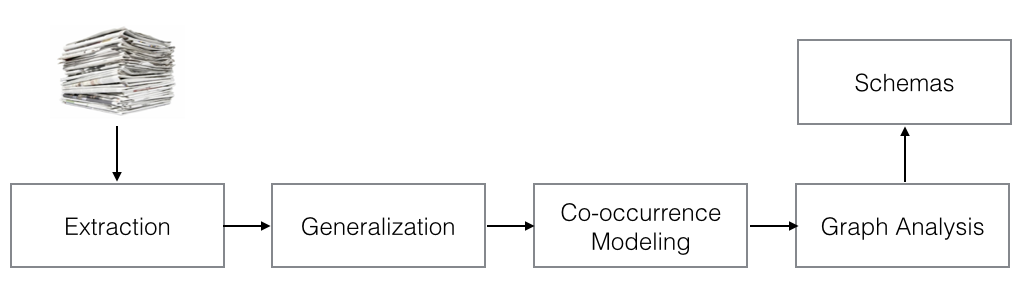
\includegraphics[height=1.75in, width=5.25in]{figures/schema-architecture}
\vspace{-4ex}
\caption{\label{fig:schema-generation}Schema Generation Pipeline}
\end{center}
\vspace{-2ex}
\end{figure}
Starting from a large collection of stories we first extract a generalized representation of the event mentions in the text. Then, we compute the co-occurrence statistics between the generalized mentions. Next, we identify relations to seed schema generation. We then construct a relation graph starting from the seed, and use graph analysis algorithms to identify the relations that belong to the schema. As a final step we resolve co-referring entities and relations and output the schema. 
There are several fundamental challenges in all stages of the pipeline. In this section, we will detail the challenges and the directions that this project will investigate for each stage.
%We use a richer representation, design techniques for generalizing arguments to an appropriate level, investigate graph-based formalisms that can effectively model sense and topic-drift issues during clustering, and build a learning-based approach for effectively scoring the generated schemas.
 
\subsection{Extraction}

The first stage in our pipeline involves extracting and representing event mentions from text. Representing information in sentences using extractions is an inherently lossy procedure. On the other hand retaining all information in a sentence doesn't scale well. Our preliminary work showed that one of the fundamental challenges in learning schemas from text is the context vs. sparsity trade-off in representation. Previous approaches used extremely limited context to represent events using (subject, verb) and (verb, object) pairs (e.g., Chambers and Jurafsky, 2009). Using such limited representations lead to incoherent schemas which mix distinct events. On the other hand, capturing more context using entire relation triples of the form (arg1, relation, arg2) leads to improved results. However, we still find that using a representation that is close to the source text has two fundamental sparsity problems: 1) Using specific mentions of events doesn't provide any generalization power. 2) Syntactic and lexical variability can mislead the system into treating the different mentions of the same event as separate events. 

To address these challenges, we propose to explore the combination of Open IE extractions with semantic role annotations. Semantic roles present a nice intermediate between ontology-free Open-IE and tight semantic ontology in closed IE systems. The thematic roles sought by SRL systems are general purpose roles that apply to a wide variety of relations. The key advantage with semantic roles is that unlike Open IE arguments, semantic role assignments are not susceptible to simple syntactic transformation and because the arguments are thematic roles, it is easy to encode N-ary relations compactly. We plan to use one of the many off-the-shelf implementations (e.g., Clear SRL~\cite{}, SemaPro~\cite{}) available\footnote{While accuracy of role labeling is important, less than perfect role labeling is not problematic in our architecture, since the roles only serve to provide a normalized argument structure -- the name of the role itself is not particularly relevant.}. 

\subsection{Generalization}

Extractions yield information about specific mentions. Generalizing from these specific mentions is the key step in extracting knowledge about types of events. This involves mapping specific instances (e.g., Barrack Obama) to an appropriate class (e.g., US President). This immediately raises two basic questions: 1) What is the underlying ontology of classes? 2) How does one map the arguments and relations to the appropriate class? For example, depending on the relation at hand {\em Barrack Obama} may map to a {\em US President}, {\em Senator}, or {\em Person}.  

{\textbf Ontology} In this work, we will leverage existing resources such as Freebase, NELL and WordNet for constructing the ontology for entities and relations. Freebase is a crowd-sourced and curated knowledge base that contains more than 43,000 types (i.e., classes)~\footnote{as of September 1st, 2014.}. Entity classification systems~\cite{xiao}, entity linking systems~\cite{tlin}, and relation extraction systems~\cite{multir} have been developed to identify instances of Freebase types. These provide a great starting 
point for mapping named entities and some subset of relations into Freebase. Events also involve common noun arguments (e.g, The fire burned down {\em the entire condominium} in 2 hours.). It is important to be able to generalize {\em condominiums} to its class {\em building}. We use Wordnet type hierarchy to assign classes to common nouns.

The ontologies, as the name implies, are hierarchies of classes. Determining what an appropriate level of generalization is a tricky problem. In our preliminary work we created multiple entires one for each type in the hierarchy up to the root. In addition to being inefficient, this method cannot be tuned to select a desired level of generalization. We propose to investigate prior work on selectional preferences and class models~\cite{} to determine the appropriate class assignment given an extraction.
 
\subsection{Co-occurrence Modeling}

This the most straight-forward piece of the pipeline, which estimates the co-occurrence probabilities of generalized event mentions. We will follow the template in our preliminary work on Rel-grams generation to produce a large table of co-occurrence frequencies and evaluate standard conditional probability estimation techniques and approaches for combining estimates obtained over different windows of document level co-occurrence. The key implementation challenge here is scaling to large collections. Rel-gram computation involves counting items that are linear in the size of the collection\footnote{With a constant proportional to the square of the average size of a document.}. We will leverage the many Map-Reduce implementation optimizations that we developed for our preliminary work.
 
\subsection{Schema Generation}

The main intuition behind schema generation is that frequently co-mentioned relations belong to the same schema and contain the salient entities and their roles. We gather frequently co-mentioned relations from the pairwise co-occurrence model. As we alluded to earlier, not all stories about an event type will mention (or necessarily) have the same set of sub-events or entities. For example, not all lawsuits will be decided in favor of the defendant and not all lawsuits will involve the filing of briefs from friends of the court, and in some cases the story itself may omit its mention. By gathering co-mentioned relations from pairwise co-occurrence models, we implicitly allow for the aggregation of information that may sometimes be missing. 

The are two main challenges in building schemas: 1) Identifying useful seeds or starting points for schemas, and 2) Effectively selecting relations to include in a schema.

\textbf{Seeding Schemas} The pairwise co-occurrences represent a large graph where the generalized relations are nodes and co-occurrences specify edge weights. In this setting, a direct approach to gathering co-mentioned relations is to perform clustering over this graph (either bottom-up or top-down). Instead we propose to investigate a seed-based expansion approach, which has several key benefits: a) Avoids the problem of large clusters resulting from hub nodes that are general purpose relations (e.g., {\em father of}, {\em spokesperson for}). b) Allows local structure around nodes to govern the inclusion in schema, which makes it easier to design selection algorithms.  c) Allows for an on-demand clustering of graph given any starting point. As we will point out later this flexibility is desirable for both development purposes (control for the seeds), as well as for use in applications which can provide an effective circumscription of the graph based on their input.

We propose to explore a probabilistic generative model for seed selection. Given a co-occurrence model with appropriate probabilistic semantics, we can directly construct a generative probabilistic model, which specifies the probability of observing other relations having observed a specific relation. The quality of a seed can be approximated by the quality of the distribution governing its neighborhood (e.g., perplexity of observing the neighboring nodes). selecting seeds that cover diverse events, as well as providing strong anchors for building schemas. 

\textbf{Graph Analysis} 

The seed-based schema generation approach has two steps.


\subsection{Contributions}

\begin{itemize}
\item Effective representation which captures adequate context to unambiguously represent event semantics. 
\item Generalization techniques that address sparsity. 
\item Graph-based approaches that leverage graphical properties to address sense and topic-drift. 
\item Scalable method for effectively scoring generated schemas. 
\end{itemize}


% !TEX root =  main.tex
\section{\label{sec:extraction} Event Extraction}

We focus on the end task of event extraction using the automatically generated schemas. The scope of this investigation will be limited to a) demonstrating the feasibility of event extraction using automatically constructed schemas, b) identifying the key issues and challenges in this application (to pursue for future work), and c) to keep the schema generation efforts grounded with respect to a specific application. 

We propose a simple bootstrapping based extension to build extractors. 
Prior template-driven extraction approaches (\cite{patwardhan-emnlp09}) use event templates to specify slots for extracting information about events or scenarios. The extraction systems were built by learning extractors for specific slots in each template. %For example, the table below shows an arrest template, which specifies the relevant pieces of extractable information about typical arrest events. 
\eat{\begin{table}[htdp]
\begin{center}
\begin{tabular}{|p{2cm}|p{8cm}|p{4cm}|}
\hline
Slot & Description & Value\\
\hline
Agent & The authority that makes the arrest. & {\em London Police}\\
Suspect & The person who was arrested. & {\em John Doe}\\
Crime & The charge under which someone is arrested. & {\em robbery}\\
Court  & The court where the suspect was produced. & {\em 8th District court, DC} \\ 
Victim & The victim of the crime & {\em Jane Eyre}\\
Lawyer & The lawyer representing the suspect. & {\em Fullerson}\\
\hline
Time & Time of arrest & Sept 18, 2014\\
Location & Place arrested & Suspect's home\\
\hline
\end{tabular}
\end{center}
\end{table}%
}

\subsection{Learning Extractors}
The schemas we generate can be used as templates since they include similar information. Recall that schemas specify the main entities and their roles as a set of generalized relations between the participants in events. Each generalized relation in a schema specifies an extraction pattern and thus the schema as a whole can be viewed as a high precision extractor. Our preliminary investigation shows that coverage of the extraction patterns is a key issue and using the schema as is will result in low recall. We propose to investigate methods that bootstrap extractors from the schemas and the original extractions that were used to construct the schemas in the first place. With each schema we have recorded the original entities, the relations, as well as the source documents from which the relations were aggregated. The documents (and smaller text spans) can be used to construct pseudo-training data by annotating the appropriate text mentions. We can then train extractors using this pseudo-training data. 

Extraction is a two-step process, which involves using the input document (text) to first identify which set of schemas can be used for extraction. Given a particular schema, we can use the individual relation extractors to identify relations and extract candidate mentions for the participants. The relations between the participants in the schema provide consistency constraints for a typical instantiation of the schema. For example, in an arrest schema, we expect that the agent of a "arrest" relation to be different from the agent of a "appeared in court" relation. Similarly, we expect that the object of the "arrest" relation to be also the object of the "charged with" relation. Finally, the extracted event can be scored using the confidences of the extractors as well as a measure of how well it satisfies the constraints specified by the schema.

\subsection{Evaluation}

We will conduct evaluations on the MUC datasets for the limited number of domains but will also conduct evaluations on a crowd-source dataset created as part of schema curation (see Section~\ref{sec:data-collection}). The evaluations will test both the mapping of schemas to the document as well as the accuracy of the extraction. The goals for evaluation are to benchmark the performance of using automatically generated schemas for event extraction and to shed light on the scalability and accuracy issues that arise in open-domain event extraction as opposed to prior MUC evaluations on a small domains. 

\subsection{Contributions}
\begin{itemize}[noitemsep,nolistsep]
\item Effective bootstrapping techniques for building extractors for schema elements.
\item Empirical evaluation of the accuracy of the extractors. 
\end{itemize}


%The main idea for extraction is to first use the general relation extraction pipeline to extract relations. Then, we identify the schema that is to be invoked given the relations in the document. A third and final step is to map the relations and their arguments into the schema and produce an aggregated extraction.

%Once we construct extractors for each relation independently, we can learn a joint extractor from the individual extractors which respects consistency constraints specified over the schema. For example, in an arrest schema, we expect that the agent of a "arrest" relation to be different from the agent of a "appeared in court" relation. Similarly, we expect that the object of the "arrest" relation to be also the object of the "charged with" relation. 


%The other key challenge in template-based event extraction is identifying the boundaries of events. Often times, multiple events of the same type are discussed. For example, a news article about a specific arson incident will often refer to previous arson incidents in the same area, which can potentially confuse extraction. This is a hard problem that is unlikely to be solved within the scope of this project.  


%\subsection{Approach}
%Schemas can be used as templates to guide extraction about events or scenarios. MUC templates have been used to drive extraction of information into pre-defined slots. For example, the following is an arrest template, which specifies slots into which entities are to be extracted.

%Schemas are a set of generalized relations between the participants in events and can be viewed as high precision extractors. Each generalized relation in a schema specifies an extraction pattern. Our preliminary work suggests that using schemas directly will result in low recall. 

%%As part of this work we will investigate methods that bootstrap extractors from the schemas. The original extractions from schemas are linked to the original extractions from which they were constructed

%Event extraction then becomes the task of aggregating the relations into event mentions. This is a two step process, where we first identify the schema that is to be invoked given the relations in the document and then mapping the relations and the entities into the schema. 

%We can construct extractors for each relation independently and then learn a joint model from the individual extractors, which respects consistency constraints specified over the schema. For example, in an arrest schema, we expect that the agent of a "arrest" relation to be different from the agent of a "appeared in court" relation. Similarly, we expect that the object of the "arrest" relation to be also the object of the "charged with" relation. 

%\subsection{Precision/Recall Trade-off}


%!TEX root = main.tex
\section{Crowd-sourcing Event Schema Curation}

One of the main obstacles to developing scalable extraction approaches is the lack of training data. Access to large scale training data covering a broad range of domains is critical for developing and evaluating approaches. We propose to overcome this limitation by using crowd-sourcing to curate the system generated schemas. There key benefit of this approach is that it requires relatively low amounts of effort to modify entries in a schema as opposed to creating new schemas from scratch. 



\subsection{Proposed Method}
Getting non-domain experts to annotate the schemas is a challenging task. We will build on the approach we used in our preliminary work, where we obtained input from Amazon Mechanical Turkers to evaluate schemas. Schemas are a complex structure with many different elements with associated type information. To reduce the evaluation burden, we sample different groundings for the participants and generated ground versions of the schema and collected judgements on these ground versions. 
Specifically we will solicit four main types of user input that cover the types of problems in automatically generated schemas:
\begin{enumerate}
\item {Correct Errors} -- There are two types of errors that we can identify and correct. First, the generalized relation may be non-sensical due to extraction errors, which is often straightforward to spot. Second, the type assignment for the arguments can be erroneous (e.g., Type: [Musician], played, Type: [Sport]). The type assignment error can be caught at the generalized relation level with the instantiated relation providing further help where needed e.g., (Michael Jackson, played, Baseball).
\item {Identify Relevant Entries} -- System generated schemas can contain completely irrelevant or topically relevant but not critical information. We will get annotations on each schema entry. Judging relevance requires a determination of the main topic of the schema. In some cases this may not be possible in which case the entire schema will be discarded.
\item {Identify Missing Entries} -- In our prior work, we noticed that while schemas tended to have high precision, the schemas could miss some important information often in domains that do not have regular reporting patterns or for scenarios that include many possible sub-events. We will explore methods for soliciting such missing information.
\item {Schema Relationships} -- We will also collect user inputs on the relationships between the automatically generated schemas. 
In keeping with our theme of minimal user inputs, we will first build an automatic method for detecting duplicates or near-duplicates.  
and get Turkers to help only on the set that the system considers as duplicates. Similarly, we will also devise methods to elicit inputs on identifying parent/child relationships between schemas.   
\end{enumerate}

As with any crowd-sourced curation effort, quality control and getting redundant inputs on the same questions will be part of our methodology. Where possible we will also utilize crowd workflows frameworks to route tasks to Turkers to maximize coverage and quality~\cite{}. We will draw upon lessons learnt from our previous attempt at crowd-sourcing schema evaluation.

\subsection{Contributions}

\begin{itemize}
\item First large scale collection of manually curated schemas. 
\item 
\end{itemize}

%% !TEX root =  main.tex
\section{\label{sec:extraction} Event Extraction}

We focus on the end task of event extraction using the automatically generated schemas. The scope of this investigation will be limited to a) demonstrating the feasibility of event extraction using automatically constructed schemas, b) identifying the key issues and challenges in this application (to pursue for future work), and c) to keep the schema generation efforts grounded with respect to a specific application. 

We propose a simple bootstrapping based extension to build extractors. 
Prior template-driven extraction approaches (\cite{patwardhan-emnlp09}) use event templates to specify slots for extracting information about events or scenarios. The extraction systems were built by learning extractors for specific slots in each template. %For example, the table below shows an arrest template, which specifies the relevant pieces of extractable information about typical arrest events. 
\eat{\begin{table}[htdp]
\begin{center}
\begin{tabular}{|p{2cm}|p{8cm}|p{4cm}|}
\hline
Slot & Description & Value\\
\hline
Agent & The authority that makes the arrest. & {\em London Police}\\
Suspect & The person who was arrested. & {\em John Doe}\\
Crime & The charge under which someone is arrested. & {\em robbery}\\
Court  & The court where the suspect was produced. & {\em 8th District court, DC} \\ 
Victim & The victim of the crime & {\em Jane Eyre}\\
Lawyer & The lawyer representing the suspect. & {\em Fullerson}\\
\hline
Time & Time of arrest & Sept 18, 2014\\
Location & Place arrested & Suspect's home\\
\hline
\end{tabular}
\end{center}
\end{table}%
}

\subsection{Learning Extractors}
The schemas we generate can be used as templates since they include similar information. Recall that schemas specify the main entities and their roles as a set of generalized relations between the participants in events. Each generalized relation in a schema specifies an extraction pattern and thus the schema as a whole can be viewed as a high precision extractor. Our preliminary investigation shows that coverage of the extraction patterns is a key issue and using the schema as is will result in low recall. We propose to investigate methods that bootstrap extractors from the schemas and the original extractions that were used to construct the schemas in the first place. With each schema we have recorded the original entities, the relations, as well as the source documents from which the relations were aggregated. The documents (and smaller text spans) can be used to construct pseudo-training data by annotating the appropriate text mentions. We can then train extractors using this pseudo-training data. 

Extraction is a two-step process, which involves using the input document (text) to first identify which set of schemas can be used for extraction. Given a particular schema, we can use the individual relation extractors to identify relations and extract candidate mentions for the participants. The relations between the participants in the schema provide consistency constraints for a typical instantiation of the schema. For example, in an arrest schema, we expect that the agent of a "arrest" relation to be different from the agent of a "appeared in court" relation. Similarly, we expect that the object of the "arrest" relation to be also the object of the "charged with" relation. Finally, the extracted event can be scored using the confidences of the extractors as well as a measure of how well it satisfies the constraints specified by the schema.

\subsection{Evaluation}

We will conduct evaluations on the MUC datasets for the limited number of domains but will also conduct evaluations on a crowd-source dataset created as part of schema curation (see Section~\ref{sec:data-collection}). The evaluations will test both the mapping of schemas to the document as well as the accuracy of the extraction. The goals for evaluation are to benchmark the performance of using automatically generated schemas for event extraction and to shed light on the scalability and accuracy issues that arise in open-domain event extraction as opposed to prior MUC evaluations on a small domains. 

\subsection{Contributions}
\begin{itemize}[noitemsep,nolistsep]
\item Effective bootstrapping techniques for building extractors for schema elements.
\item Empirical evaluation of the accuracy of the extractors. 
\end{itemize}


%The main idea for extraction is to first use the general relation extraction pipeline to extract relations. Then, we identify the schema that is to be invoked given the relations in the document. A third and final step is to map the relations and their arguments into the schema and produce an aggregated extraction.

%Once we construct extractors for each relation independently, we can learn a joint extractor from the individual extractors which respects consistency constraints specified over the schema. For example, in an arrest schema, we expect that the agent of a "arrest" relation to be different from the agent of a "appeared in court" relation. Similarly, we expect that the object of the "arrest" relation to be also the object of the "charged with" relation. 


%The other key challenge in template-based event extraction is identifying the boundaries of events. Often times, multiple events of the same type are discussed. For example, a news article about a specific arson incident will often refer to previous arson incidents in the same area, which can potentially confuse extraction. This is a hard problem that is unlikely to be solved within the scope of this project.  


%\subsection{Approach}
%Schemas can be used as templates to guide extraction about events or scenarios. MUC templates have been used to drive extraction of information into pre-defined slots. For example, the following is an arrest template, which specifies slots into which entities are to be extracted.

%Schemas are a set of generalized relations between the participants in events and can be viewed as high precision extractors. Each generalized relation in a schema specifies an extraction pattern. Our preliminary work suggests that using schemas directly will result in low recall. 

%%As part of this work we will investigate methods that bootstrap extractors from the schemas. The original extractions from schemas are linked to the original extractions from which they were constructed

%Event extraction then becomes the task of aggregating the relations into event mentions. This is a two step process, where we first identify the schema that is to be invoked given the relations in the document and then mapping the relations and the entities into the schema. 

%We can construct extractors for each relation independently and then learn a joint model from the individual extractors, which respects consistency constraints specified over the schema. For example, in an arrest schema, we expect that the agent of a "arrest" relation to be different from the agent of a "appeared in court" relation. Similarly, we expect that the object of the "arrest" relation to be also the object of the "charged with" relation. 

%\subsection{Precision/Recall Trade-off}


%% !TEX root =  main.tex
\section{Salience and Dependence Models}

\subsection{Salience}

\subsection{Dependence}

\textbf{Not temporal} but dependence as it simplifies the needs with respect to end tasks (temporal ordering of events is useful in its own right) but that is not the focus here.

\textbf{What features to use?}

\subsection{Evaluation}

\textbf{Intrinsic evaluation} via predictive tasks. 


\subsection{Contributions}
\begin{itemize}
\item Formal models for estimating salience and dependence.
\item Empirical evaluation of the intrinsic quality of the models. 
\end{itemize}
%% !TEX root =  main.tex
\section{Applications and Schema Refinement}

\subsection{Event Extraction}
\textbf{System Diagram?}

\subsection{Summarization}

\textbf{Why should event schemas help?}

\subsection{Other Applications}

Entity linking and Reference resolution???


\subsection{Refinement}


\subsection{Contributions}

\begin{itemize}
\item Benchmark performance on end tasks.
\item Method for mapping schemas to a given document.
\item Task-driven adaptations for salience and dependence model estimation.
\end{itemize}
% !TEX root =  main.tex
\section{Development Plan and Timeline}

The project will proceed in three phases. In the first phase of the project, we focus on the designing the representation and extracting information from large corpora using existing IE systems. We will design a rich representation for the targeted knowledge by leveraging existing ontologies for entities and relations (e.g., YAGO, NELL, Freeebase) where possible and using text derived representations in other places. Then, we will investigate techniques for aggregating and generalizing information in the specific instances. In particular, we will develop automatic methods for choosing the right level for mapping into a type hierarchy for the arguments and the relations. In the second phase, we will focus on graph-based approaches for generating open-domain schemas using the generalized extractions. In our preliminary work, we identified the graph properties that indicate specific characteristics for good schemas and developed a suitable method that exploited the graph properties to produce high-quality schemas. In the third phase, we will focus on applying the generated schemas to two end tasks: event extraction, and summarization. For event extraction we will build extractors. Schemas can be thought of as high-precision models of events, which can then be expanded to include higher-recall extractors via bootstrapping. For summarization, we will use schemas to help select sentences for the standard MUC single document summarization task. We will iterate and refine the schema representation and generation based on their performance in these end tasks.

Year 1:  
\begin{enumerate}
\item Design target Representation for Knowledge  Design representation manually based on use cases from target applications.
\item Information Extraction and Aggregating existing knowledge. Annotate documents using Open IE and link entities to existing resources. Explore Generalization Techniques 
� Develop methods for generalize specific instances (e.g., John was arrested in Bristol, UK �> [Person] arrested in [Location])
\item Construct micro-theories using corpus analysis. Co-mentioned (and argument sharing) instances are likely part of some theory. Mechanical Turk Evaluation of Micro-Theories.
\end{enumerate}

Year 2:
\begin{enumerate}
\item Relate micro-theories to each other 
\item Inference over graphs to enhance recall and precision of theories..
\item Iterative development w/ target application: 1) Apply learned theories to target application. 2) Recall is often an issue. Explore on demand construction of theory given a particular document. 
\end{enumerate}


\section{Broader Impact}

Event schemas directly impact many practical applications and provide a stepping stone for advances in knowledge-intensive AI applications. Businesses gather ever increasing amounts of data from customers and users via social platforms, analysts deal with increasing news volumes, researchers produce and consume vast amounts of knowledge through publications. All these diverse communities can benefit from scalable information extraction and summarization systems. Event schemas are an important step towards automatically building script-like knowledge from text, which can benefit knowledge-intensive AI applications such as reasoning and Question Answering. Furthermore, the method and techniques can scale to other domains and spur research on similar problems (e.g., extracting processes from textbooks, identifying schemas in research studies).

\section{Curriculum Development Activities}

I plan to teach a course centered around the core concepts of scalable information extraction and knowledge extraction techniques. 
Most technology companies with a large web presence have a need for extracting information of one form or other from information obtained by engaging with their user base. This course will provide a basic overview of a distributed information extraction pipeline, persistence, and building applications that rely on the extracted data. 

\section{Prior NSF Support}

\section{Data Management Plan}

 
{\small
\bibliographystyle{plain}
\bibliography{kia,main}
}
\end{document}
